\documentclass{standalone}
\usepackage{tikz}
\usetikzlibrary{patterns, positioning}


\begin{document}
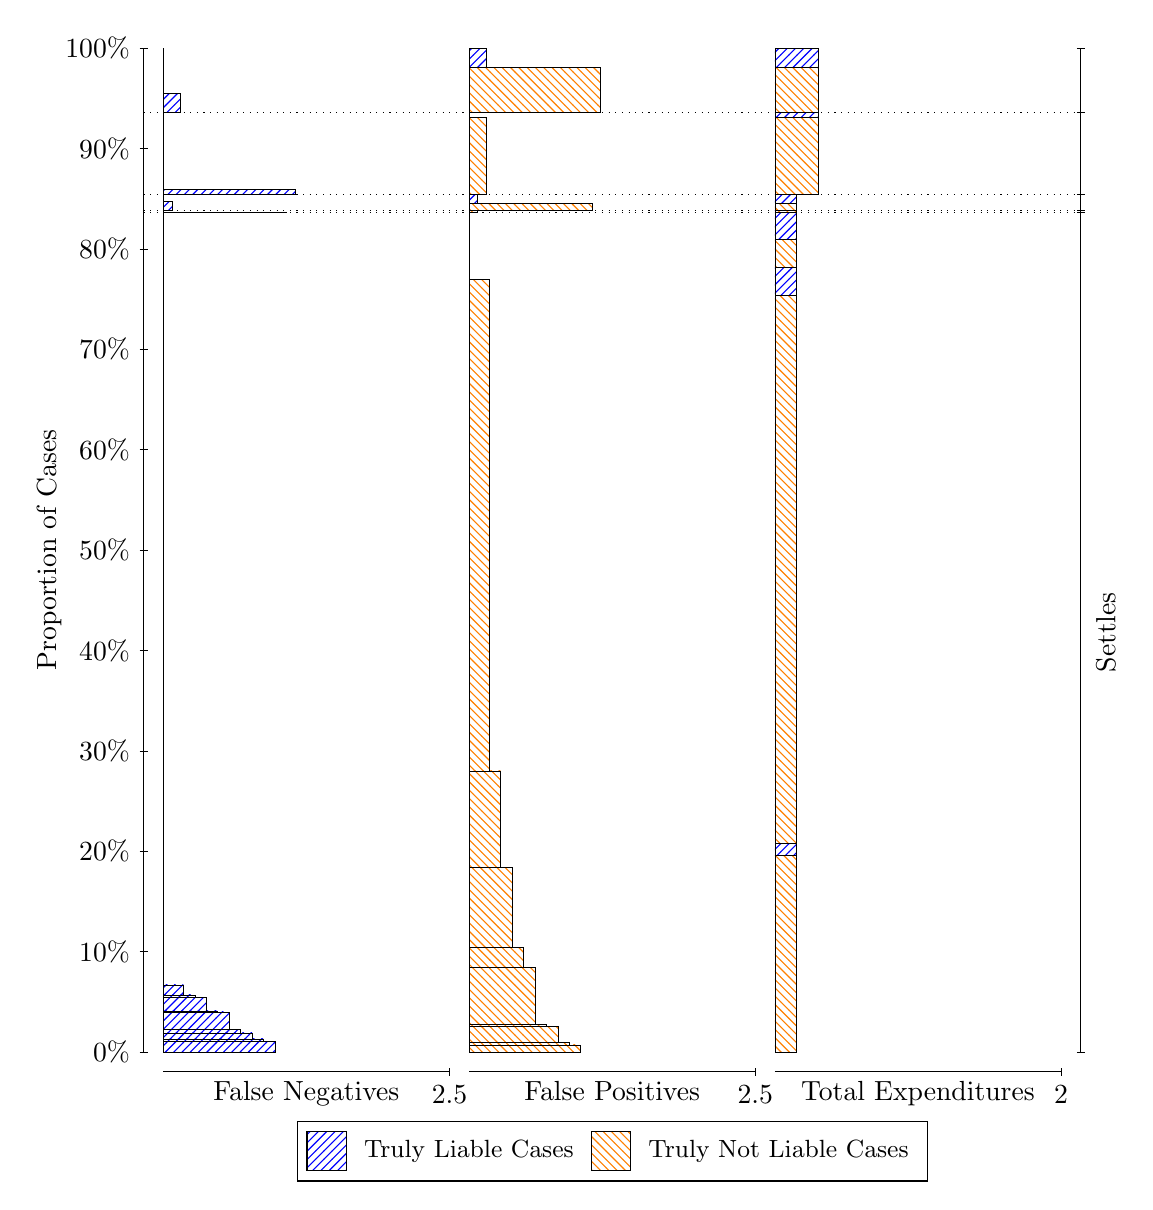
\begin{tikzpicture}
\draw[black, very thin] (1.5,1.75) -- (1.5,14.5);
\node[rotate=90, text=black, anchor=center] at (0.3, 8.125) {Proportion of Cases};
\draw[black, very thin] (1.45,1.75) -- (1.55,1.75);
\node[text=black, anchor=east] at (1.45, 1.75) {0\%};
\draw[black, very thin] (1.45,3.025) -- (1.55,3.025);
\node[text=black, anchor=east] at (1.45, 3.025) {10\%};
\draw[black, very thin] (1.45,4.3) -- (1.55,4.3);
\node[text=black, anchor=east] at (1.45, 4.3) {20\%};
\draw[black, very thin] (1.45,5.575) -- (1.55,5.575);
\node[text=black, anchor=east] at (1.45, 5.575) {30\%};
\draw[black, very thin] (1.45,6.85) -- (1.55,6.85);
\node[text=black, anchor=east] at (1.45, 6.85) {40\%};
\draw[black, very thin] (1.45,8.125) -- (1.55,8.125);
\node[text=black, anchor=east] at (1.45, 8.125) {50\%};
\draw[black, very thin] (1.45,9.4) -- (1.55,9.4);
\node[text=black, anchor=east] at (1.45, 9.4) {60\%};
\draw[black, very thin] (1.45,10.675) -- (1.55,10.675);
\node[text=black, anchor=east] at (1.45, 10.675) {70\%};
\draw[black, very thin] (1.45,11.95) -- (1.55,11.95);
\node[text=black, anchor=east] at (1.45, 11.95) {80\%};
\draw[black, very thin] (1.45,13.225) -- (1.55,13.225);
\node[text=black, anchor=east] at (1.45, 13.225) {90\%};
\draw[black, very thin] (1.45,14.5) -- (1.55,14.5);
\node[text=black, anchor=east] at (1.45, 14.5) {100\%};

\draw[black, very thin] (13.4,1.75) -- (13.4,14.5);
\draw[black, very thin] (13.35,1.75) -- (13.45,1.75);
\node[anchor=west] at (13.35, 1.75) {};
\draw[black, very thin] (13.35,12.413) -- (13.45,12.413);
\node[anchor=west] at (13.35, 12.413) {};
\draw[black, very thin] (13.35,12.436) -- (13.45,12.436);
\node[anchor=west] at (13.35, 12.436) {};
\draw[black, very thin] (13.35,12.641) -- (13.45,12.641);
\node[anchor=west] at (13.35, 12.641) {};
\draw[black, very thin] (13.35,13.678) -- (13.45,13.678);
\node[anchor=west] at (13.35, 13.678) {};
\draw[black, very thin] (13.35,14.5) -- (13.45,14.5);
\node[anchor=west] at (13.35, 14.5) {};

\draw[black, very thin, pattern color=blue, pattern=north east lines] (1.75,1.75) rectangle (3.167,1.883);
\draw[black, very thin, pattern color=blue, pattern=north east lines] (1.75,1.883) rectangle (3.0217,1.9165);
\draw[black, very thin, pattern color=blue, pattern=north east lines] (1.75,1.9165) rectangle (2.8763,1.9913);
\draw[black, very thin, pattern color=blue, pattern=north east lines] (1.75,1.9913) rectangle (2.731,2.034);
\draw[black, very thin, pattern color=blue, pattern=north east lines] (1.75,2.034) rectangle (2.5857,2.2587);
\draw[black, very thin, pattern color=blue, pattern=north east lines] (1.75,2.2587) rectangle (2.4403,2.2718);
\draw[black, very thin, pattern color=blue, pattern=north east lines] (1.75,2.2718) rectangle (2.295,2.4454);
\draw[black, very thin, pattern color=blue, pattern=north east lines] (1.75,2.4454) rectangle (2.1497,2.4749);
\draw[black, very thin, pattern color=blue, pattern=north east lines] (1.75,2.4749) rectangle (2.0043,2.6014);
\draw[black, very thin, pattern color=orange, pattern=north west lines] (1.75,2.6014) rectangle (1.75,12.413);
\draw[black, very thin, pattern color=blue, pattern=north east lines] (1.75,12.413) rectangle (3.3123,12.414);
\draw[black, very thin, pattern color=orange, pattern=north west lines] (1.75,12.414) rectangle (1.75,12.436);
\draw[black, very thin, pattern color=blue, pattern=north east lines] (1.75,12.436) rectangle (1.859,12.549);
\draw[black, very thin, pattern color=orange, pattern=north west lines] (1.75,12.549) rectangle (1.75,12.641);
\draw[black, very thin, pattern color=blue, pattern=north east lines] (1.75,12.641) rectangle (3.4213,12.704);
\draw[black, very thin, pattern color=orange, pattern=north west lines] (1.75,12.704) rectangle (1.75,13.678);
\draw[black, very thin, pattern color=blue, pattern=north east lines] (1.75,13.678) rectangle (1.968,13.924);
\draw[black, very thin, pattern color=orange, pattern=north west lines] (1.75,13.924) rectangle (1.75,14.5);
\draw[black, very thin, pattern color=orange, pattern=north west lines] (5.6333,1.75) rectangle (7.0503,1.8413);
\draw[black, very thin, pattern color=orange, pattern=north west lines] (5.6333,1.8413) rectangle (6.905,1.8699);
\draw[black, very thin, pattern color=orange, pattern=north west lines] (5.6333,1.8699) rectangle (6.7597,2.0794);
\draw[black, very thin, pattern color=orange, pattern=north west lines] (5.6333,2.0794) rectangle (6.6143,2.1042);
\draw[black, very thin, pattern color=orange, pattern=north west lines] (5.6333,2.1042) rectangle (6.469,2.8201);
\draw[black, very thin, pattern color=orange, pattern=north west lines] (5.6333,2.8201) rectangle (6.3237,3.0826);
\draw[black, very thin, pattern color=orange, pattern=north west lines] (5.6333,3.0826) rectangle (6.1783,4.0973);
\draw[black, very thin, pattern color=orange, pattern=north west lines] (5.6333,4.0973) rectangle (6.033,5.3206);
\draw[black, very thin, pattern color=orange, pattern=north west lines] (5.6333,5.3206) rectangle (5.8877,11.562);
\draw[black, very thin, pattern color=blue, pattern=north east lines] (5.6333,11.562) rectangle (5.6333,12.413);
\draw[black, very thin, pattern color=orange, pattern=north west lines] (5.6333,12.413) rectangle (5.7423,12.435);
\draw[black, very thin, pattern color=blue, pattern=north east lines] (5.6333,12.435) rectangle (5.6333,12.436);
\draw[black, very thin, pattern color=orange, pattern=north west lines] (5.6333,12.436) rectangle (7.1957,12.527);
\draw[black, very thin, pattern color=blue, pattern=north east lines] (5.6333,12.527) rectangle (5.7423,12.641);
\draw[black, very thin, pattern color=orange, pattern=north west lines] (5.6333,12.641) rectangle (5.8513,13.615);
\draw[black, very thin, pattern color=blue, pattern=north east lines] (5.6333,13.615) rectangle (5.6333,13.678);
\draw[black, very thin, pattern color=orange, pattern=north west lines] (5.6333,13.678) rectangle (7.3047,14.254);
\draw[black, very thin, pattern color=blue, pattern=north east lines] (5.6333,14.254) rectangle (5.8513,14.5);
\draw[black, very thin, pattern color=orange, pattern=north west lines] (9.5167,1.75) rectangle (9.7892,4.2506);
\draw[black, very thin, pattern color=blue, pattern=north east lines] (9.5167,4.2506) rectangle (9.7892,4.4016);
\draw[black, very thin, pattern color=orange, pattern=north west lines] (9.5167,4.4016) rectangle (9.7892,11.359);
\draw[black, very thin, pattern color=blue, pattern=north east lines] (9.5167,11.359) rectangle (9.7892,11.717);
\draw[black, very thin, pattern color=orange, pattern=north west lines] (9.5167,11.717) rectangle (9.7892,12.071);
\draw[black, very thin, pattern color=blue, pattern=north east lines] (9.5167,12.071) rectangle (9.7892,12.413);
\draw[black, very thin, pattern color=orange, pattern=north west lines] (9.5167,12.413) rectangle (9.7892,12.435);
\draw[black, very thin, pattern color=blue, pattern=north east lines] (9.5167,12.435) rectangle (9.7892,12.436);
\draw[black, very thin, pattern color=orange, pattern=north west lines] (9.5167,12.436) rectangle (9.7892,12.527);
\draw[black, very thin, pattern color=blue, pattern=north east lines] (9.5167,12.527) rectangle (9.7892,12.641);
\draw[black, very thin, pattern color=orange, pattern=north west lines] (9.5167,12.641) rectangle (10.062,13.615);
\draw[black, very thin, pattern color=blue, pattern=north east lines] (9.5167,13.615) rectangle (10.062,13.678);
\draw[black, very thin, pattern color=orange, pattern=north west lines] (9.5167,13.678) rectangle (10.062,14.254);
\draw[black, very thin, pattern color=blue, pattern=north east lines] (9.5167,14.254) rectangle (10.062,14.5);
\draw[black, dotted] (1.5,12.413) -- (13.4,12.413);
\draw[black, dotted] (1.5,12.436) -- (13.4,12.436);
\draw[black, dotted] (1.5,12.641) -- (13.4,12.641);
\draw[black, dotted] (1.5,13.678) -- (13.4,13.678);
\draw[black, very thin] (1.75,1.5) -- (5.3833,1.5);
\node[text=black, anchor=north] at (3.5667, 1.5) {False Negatives};
\draw[black, very thin] (5.3833,1.45) -- (5.3833,1.55);
\node[text=black, anchor=north] at (5.3833, 1.45) {2.5};

\draw[black, very thin] (5.6333,1.5) -- (9.2667,1.5);
\node[text=black, anchor=north] at (7.45, 1.5) {False Positives};
\draw[black, very thin] (9.2667,1.45) -- (9.2667,1.55);
\node[text=black, anchor=north] at (9.2667, 1.45) {2.5};

\draw[black, very thin] (9.5167,1.5) -- (13.15,1.5);
\node[text=black, anchor=north] at (11.333, 1.5) {Total Expenditures};
\draw[black, very thin] (13.15,1.45) -- (13.15,1.55);
\node[text=black, anchor=north] at (13.15, 1.45) {2};

\node[text=black, centered, rotate=90] at (13.72, 7.0817) {Settles};





\draw (7.449999999999999,1.5) node[draw=none] (baseCoordinate) {};
\begin{scope}[align=center]
        \matrix[scale=0.5, draw=black, below=0.5cm of baseCoordinate, nodes={draw}, column sep=0.1cm]{
            \node[rectangle, draw, minimum width=0.5cm, minimum height=0.5cm, pattern color=blue, pattern=north east lines] {}; &
            \node[draw=none, font=\small, text=black] (B) {Truly Liable Cases}; &
            \node[rectangle, draw, minimum width=0.5cm, minimum height=0.5cm, pattern color=orange, pattern=north west lines] {}; &
            \node[draw=none, font=\small, text=black] (B) {Truly Not Liable Cases}; \\
            };
\end{scope}

\end{tikzpicture}
\end{document}